% Created 2012-07-06 Fr 12:01
\documentclass[bigger]{beamer}
\usepackage[utf8]{inputenc}
\usepackage[T1]{fontenc}
\usepackage{fixltx2e}
\usepackage{graphicx}
\usepackage{longtable}
\usepackage{float}
\usepackage{wrapfig}
\usepackage{soul}
\usepackage{textcomp}
\usepackage{marvosym}
\usepackage{wasysym}
\usepackage{latexsym}
\usepackage{amssymb}
\usepackage{hyperref}
\tolerance=1000
\usepackage{color}
\usepackage{listings}
\institute{\url{http://berndweiss.net} \\ \url{bernd.weiss@uni-koeln.de}}
\mode<beamer>{\usecolortheme{seagull}}
\usepackage{attrib}
\usepackage[T1]{fontenc}
\usepackage{tikz}
\usepackage[english]{babel}
\usepackage{graphicx}
\usepackage{tabularx}
\usepackage{amsmath}
\usepackage{bm}
\usepackage[babel]{csquotes}
\usepackage{blindtext} 
\usepackage{helvet} %\usepackage{lucidabr}
\AtBeginSection[]{ \begin{frame} \frametitle{Topic} \begin{footnotesize} \tableofcontents[currentsection, currentsubsection] \end{footnotesize} \end{frame} }
\AtBeginSubsection[]{ \begin{frame} \frametitle{Topic} \begin{footnotesize} \tableofcontents[currentsection, currentsubsection] \end{footnotesize} \end{frame} }
\hypersetup{colorlinks=true, urlcolor=cyan, linkcolor=black}
\providecommand{\alert}[1]{\textbf{#1}}

\title{\enquote{Reproducible Research} mit \newline Emacs' Org mode und R}
\author{Bernd Weiß}
\date{\footnotesize{2012-07-06}}
\hypersetup{
  pdfkeywords={},
  pdfsubject={},
  pdfcreator={Emacs Org-mode version 7.8.11}}

\begin{document}

\maketitle

\begin{frame}
\frametitle{Outline}
\setcounter{tocdepth}{3}
\tableofcontents
\end{frame}


















\definecolor{dkgreen}{rgb}{0,0.5,0}
\definecolor{dkred}{rgb}{0.5,0,0}
\definecolor{gray}{rgb}{0.5,0.5,0.5}

\lstset{basicstyle=\ttfamily\bfseries\footnotesize,
morekeywords={virtualinvoke},
%%keywordstyle=\color{blue},
%%ndkeywordstyle=\color{red},
commentstyle=\color{dkred},
%%stringstyle=\color{dkgreen},
numbers=left,
numberstyle=\ttfamily\tiny\color{gray},
stepnumber=1,
numbersep=10pt,
backgroundcolor=\color{white},
tabsize=4,
showspaces=false,
showstringspaces=false,
xleftmargin=.23in
}




\section{Vorbemerkungen}
\label{sec-1}
\subsection{}
\begin{frame}
\frametitle{Vorbemerkungen}
\label{sec-1-1-1}

\begin{itemize}
\item Bin fortgeschrittener Anfänger was Org angeht
\item Vielen Dank an Carsten Dominik (von 2003 bis 2011 Hauptentwickler), Eric Schulte und Dan Davison
  (haben die \enquote{Babel-Funktionen} in Org Mode entwickelt)
\item Alle Materialien (inkl. engl. Fassung der Folien) dieser Präsentation finden sich auf github: \href{https://github.com/berndweiss/ps2012-07-KRUG_org_r}{https://github.com/berndweiss/ps2012-07-KRUG\_org\_r}.
\end{itemize}
\end{frame}
\section{Einleitung}
\label{sec-2}
\subsection{Problem}
\label{sec-2-1}
\begin{frame}
\frametitle{Problem}
\label{sec-2-1-1}


\begin{itemize}
\item Das Verfassen eines empirischen (Forschungs-)Artikels
\begin{itemize}
\item ist selten ein linearer Prozess.
\item ist außerdem mit dem Problem verbunden, dass die wissenschaftliche
    Gemeinschaft meinen Ausführungen vertrauen können muss. Doch wie schaffe ich
    dieses Vertrauen?
\end{itemize}
\item Wir benötigen zum Verfassen eines Artikels also ein Tool, das
\begin{itemize}
\item \enquote{dynamische Elemente} enthält. Wenn sich die Datengrundlage ändert, sorgen
    diese \enquote{dynamischen Elemente} dafür, dass etwa alle Tabellen oder Abbildungen
    erneuert werden.
\item vollständigen Zugang zum Analysecode ermöglicht und damit auch Replikationen (i.e. \enquote{reproducible research}).
\end{itemize}
\end{itemize}
\end{frame}
\begin{frame}
\frametitle{Literate programming und reproducible research}
\label{sec-2-1-2}


\begin{description}
\item[\textbf{Literate programming (LP)}] Enhances traditional software development by
     embedding code in explanatory essays and encourages treating the
     act of development as one of communication with future
     maintainers.
\item[\textbf{Reproducible research (RR)}] Embeds executable code in research reports
     and publications, with the aim of allowing readers to re-run the
     analyses described.
\end{description}

     
(Source: Schulte et al. 2012: 3)
\end{frame}
\begin{frame}
\frametitle{Existing tools}
\label{sec-2-1-3}



\begin{center}
\begin{tabular}{l|ccccc}
                                       &           &       &  \LaTeX{}  &  HTML    &                                                               \\
 Tool                                  &  LP       &  RR   &  Export    &  Export  &  Language                                                     \\
\hline
 \hyperref[latex-proglang]{Javadoc}    &  partial  &  no   &  no        &  yes     &  \hyperref[latex-proglang]{Java}                              \\
 \hyperref[latex-proglang]{POD}        &  partial  &  no   &  no        &  yes     &  \hyperref[latex-proglang]{Perl}                              \\
 \hyperref[latex-proglang]{Haskell}    &  partial  &  no   &  yes       &  yes     &  \hyperref[latex-proglang]{Haskell}                           \\
 \hyperref[latex-proglang]{noweb}      &  yes      &  no   &  yes       &  yes     &  any                                                          \\
 \hyperref[latex-proglang]{cweb}       &  yes      &  no   &  yes       &  yes     &  \hyperref[latex-proglang]{C}/\hyperref[latex-proglang]{C++}  \\
 \hyperref[latex-proglang]{Sweave}     &  partial  &  yes  &  yes       &  yes     &  \hyperref[latex-proglang]{R}                                 \\
 \hyperref[latex-proglang]{SASweave}   &  partial  &  yes  &  yes       &  yes     &  \hyperref[latex-proglang]{R}/\hyperref[latex-proglang]{SAS}  \\
 \hyperref[latex-proglang]{Statweave}  &  partial  &  yes  &  yes       &  yes     &  any                                                          \\
 \hyperref[latex-proglang]{Scribble}   &  yes      &  yes  &  yes       &  yes     &  \hyperref[latex-proglang]{scheme}                            \\
 Knitr                                 &  partial  &  yes  &  yes       &  yes     &  R                                                            \\
 dexy                                  &  yes      &  yes  &  yes       &  yes     &  any                                                          \\
 \hyperref[latex-proglang]{Org-mode}   &  yes      &  yes  &  yes       &  yes     &  any                                                          \\
\end{tabular}
\end{center}



(Source: Schulte et al. 2012: 6, modified and updated)
\end{frame}
\subsection{Emacs}
\label{sec-2-2}
\begin{frame}
\frametitle{Emacs -- ein kurzer Überblick}
\label{sec-2-2-1}

\begin{itemize}
\item Emacs ist a Texteditor
\item Erweiterbar und an eigene Bedürfnisse anpassbar durch Emacs Lisp
\item Emacs steht für \enquote{Editor MACroS}
\item Entwicklung begann bereits in den 1970er Jahren, die aktuelle Version ist 24.1
\item Ich nutze Emacs vor allem für R und \LaTeX
\item Emacs kennt sg. \enquote{content-sensitive} editing (major and minor) \emph{modes}
  (u.a. für R, \LaTeX, C, C++, Python, plain text, HTML, \ldots{})
\end{itemize}

(Source: \href{http://www.gnu.org/software/emacs/}{http://www.gnu.org/software/emacs/}, \href{http://en.wikipedia.org/wiki/Emacs}{http://en.wikipedia.org/wiki/Emacs})
\end{frame}
\begin{frame}
\frametitle{Screen shot einer Emacs session}
\label{sec-2-2-2}


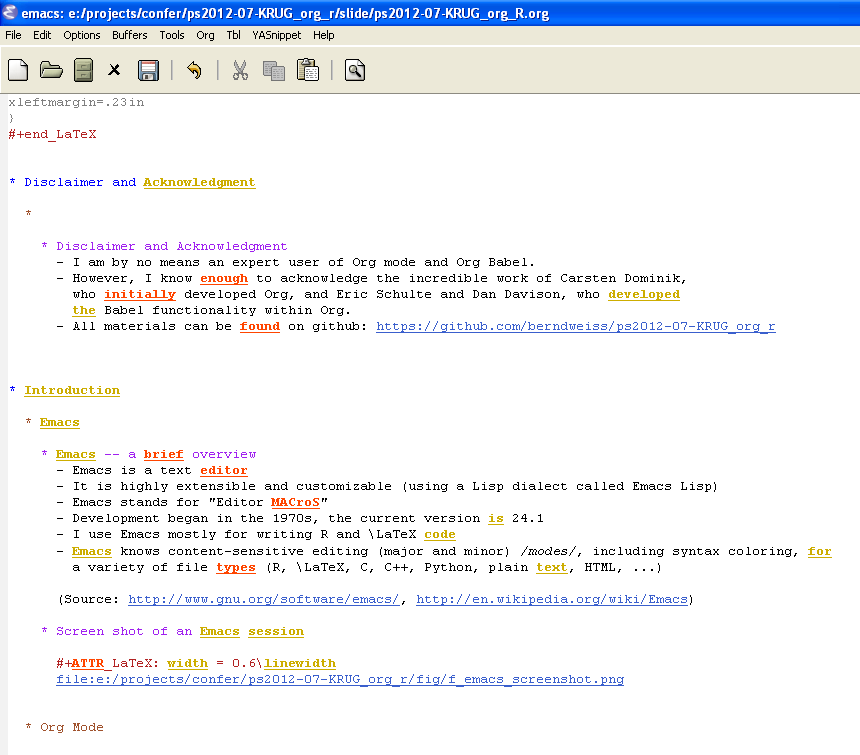
\includegraphics[width = 0.8\linewidth]{e:/projects/confer/ps2012-07-KRUG_org_r/fig/f_emacs_screenshot.png}
\end{frame}
\subsection{Org mode}
\label{sec-2-3}
\begin{frame}
\frametitle{Org mode}
\label{sec-2-3-1}

\begin{itemize}
\item Org ist ein \enquote{Emacs (major) mode for notes, planning, and authoring}
\item Org files sind plain-text files
\item Ich nutze Org für
\begin{itemize}
\item technische Dokumentationen (Export nach PDF via pdfLaTeX or HTML) oder zur
    Erstellung von Folien
\item Organisation meines beruflichen und privaten Lebens (Verabredungen,
    Todo-Listen etc.)
\item Für meine persönliche Wissensdatenbank
\item \ldots{}
\end{itemize}
\item Mehr unter: \href{http://www.orgmode.org}{http://www.orgmode.org} (tutorials, videos, \ldots{})
\end{itemize}
\end{frame}
\begin{frame}[fragile,shrink = 25]
\frametitle{Ein Org-Beispiel (source file)}
\label{sec-2-3-2}



\lstset{language=org}
\begin{lstlisting}
#+TITLE: Hello World!
#+AUTHOR: Martin Mosquito
#+DATE: <2012-07-06 Fr>

\thispagestyle{empty}

* Headline

  Lorem ipsum dolor sit amet, consetetur sadipscing elitr, sed 
  diam nonumy eirmod tempor invidunt ut labore et dolore magna 
  aliquyam erat, sed diam voluptua. At vero eos et accusam et 
  justo duo dolores et ea rebum. Stet clita kasd gubergren, no 
  sea takimata sanctus est Lorem ipsum dolor sit. 

  A list:
  - Item 1
  - Item 2  

** Subsection 

   Lorem ipsum dolor sit amet, consetetur sadipscing elitr, 
   sed diam nonumy eirmod tempor invidunt ut labore et dolore 
   magna aliquyam erat, sed diam
   
   \begin{equation}
   y = \alpha + \beta_1 x_1 + \epsilon
   \end{equation}
\end{lstlisting}
\end{frame}
\begin{frame}
\frametitle{Ein Org-Beispiel (exported to PDF)}
\label{sec-2-3-3}


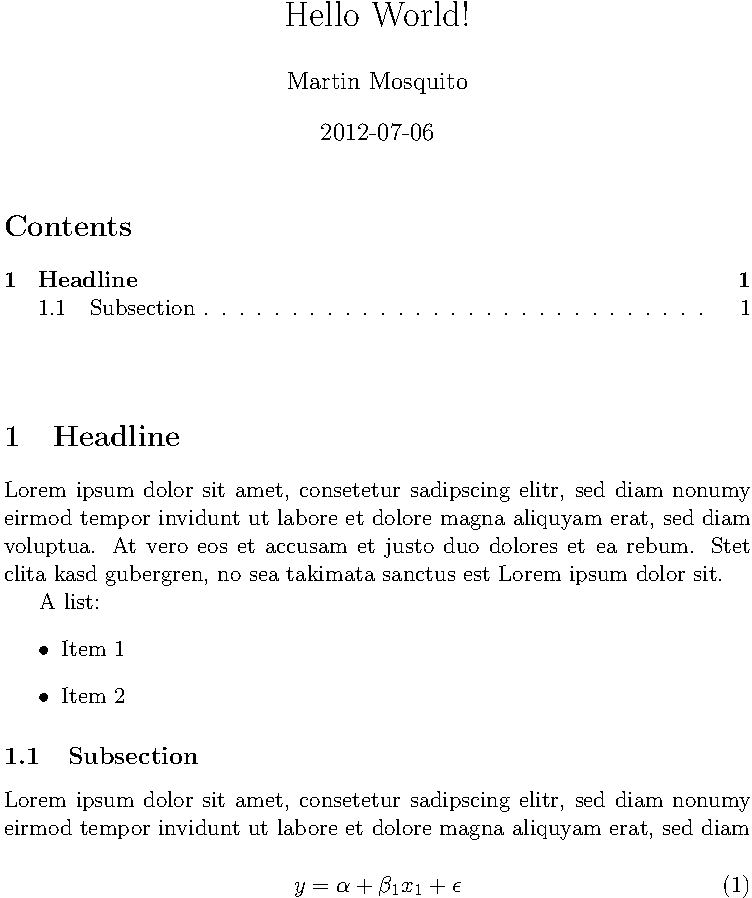
\includegraphics[clip, width = 0.6\linewidth]{e:/projects/confer/ps2012-07-KRUG_org_r/fig/org_example.pdf}
\end{frame}
\subsection{Babel: Active code in Org mode}
\label{sec-2-4}
\begin{frame}
\frametitle{Babel: Active code in Org mode}
\label{sec-2-4-1}


\begin{quote}
Babel is about letting many different languages work together. Programming languages live in blocks inside natural language Org-mode documents. A piece of data may pass from a table to a Python code block, then maybe move on to an R code block, and finally end up embedded as a value in the middle of a paragraph or possibly pass through a gnuplot code block and end up as a plot embedded in the document.
\end{quote}

(Source: \href{http://orgmode.org/worg/org-contrib/babel/intro.html}{http://orgmode.org/worg/org-contrib/babel/intro.html})
\end{frame}
\begin{frame}[fragile]
\frametitle{Using code with(in) Org mode}
\label{sec-2-4-2}


  \usetikzlibrary{shapes,arrows,shadows,decorations,decorations.text,through}
  \tikzstyle{page} = [rectangle, draw, text width=9em,
  text centered, rounded corners,
  node distance=3cm, minimum height=1em,
  font=\tiny,
  fill=blue!20,
  general shadow={
    fill=black!30,
    shadow xshift=0.16cm,
    shadow yshift=-0.16cm
  },
  very thick,
  draw=blue]
  \begin{figure}[t!]
    \centering

%% Scale TIkZ figure
%% Source: http://stackoverflow.com/questions/2239328/control-font-size-in-graphics-in-latex-when-scaling-in-minipage-subfig
    \begin{tikzpicture}[->,>=stealth', shorten >=1pt, auto, transform canvas={scale=0.55}]
      \node [page] (org) at (0,0) {
        \begin{center}
          \normalsize{Org-mode}
        \end{center}
  \begin{verbatim}
    * Plain Text Markup
    - prose composition
    - code composition
    - data analysis

  ,  #+begin_src C :tangle run.c
      int main(){
        return 0;
      }
  ,  #+end_src

  ,  #+headers: :results graphics
  ,  #+begin_src R :file fig.pdf
      plot(data)
  ,  #+end_src

  \end{verbatim}
      };

      \node [page] (htm) at (8,1) {
        \begin{center}
          \normalsize{HTML}
        \end{center}
  \begin{verbatim}
    <h1>Plain Text Markup</h1>
    <ul>
    <li>prose composition</li>
    <li>code composition</li>
    <li>data analysis</li>
    </ul>
  \end{verbatim}
      };

      \node [page] (tex) at (9,-1) {
        \begin{center}
          \normalsize{\LaTeX{}}
        \end{center}
  \begin{verbatim}
    \Section{Plain Text Markup}
    \begin{itemize}
    \item prose composition
    \item code composition
    \item data analysis
    \end{itemize}
  \end{verbatim}
      };

      \node [page, text width=6.5em] (src) at (-8,0) {
        \begin{center}
          \normalsize{Source Code}
        \end{center}
  \begin{verbatim}
    int main(){
      return 0;
    }
  \end{verbatim}
      };

      \node [text width=8em] (code-out) at (4,-6) {Embedded data and
        source code in arbitrary\\ languages};

      \node [text width=8em] (code-out) at (-4,-6) {Raw output,
        tabular data, figures, etc.};

      \path (org) edge [loop below] node {\small{Code Evaluation}} (
      \path (org) edge node {\small{Export}} (5.25,0);
      \path (org) edge node [above, text width=4.25em] {\small{Code\\  Extraction}} (-5.875,0);
      \path (org) edge node [below] {\small{(Weave)}} (5.25,0);
      \path (org) edge node [below] {\small{(Tangle)}} (-5.875,0);
    \end{tikzpicture}
  \end{figure}
\vspace{3cm}
\vfill
Source: Schulte et al. (2012)
\end{frame}
\section{Babel und R}
\label{sec-3}
\subsection{Einführung}
\label{sec-3-1}
\begin{frame}[fragile]
\frametitle{Syntax eines Org-Code-Blocks}
\label{sec-3-1-1}


\begin{small}

\begin{verbatim}
#+NAME: <name>
#+BEGIN_SRC <language> <switches> <header arguments>
 <body>
#+END_SRC
\end{verbatim}
\end{small}
\end{frame}
\begin{frame}[fragile,t, shrink = 15]
\frametitle{R code blocks I (exports code and results)}
\label{sec-3-1-2}
\begin{block}{R code block}
\label{sec-3-1-2-1}


\begin{verbatim}
This is a short sentence. This is another sentence. 
And, finally, here comes some R code:

#+BEGIN_SRC R
set.seed(1)
x1 <- rnorm(100) 
mean(x1) 
x1.sd <- sd(x1) 
#+END_SRC

#+RESULTS:
: [1] 0.1088874
\end{verbatim}
\end{block}
\begin{block}{Evaluated and exported R code block}
\label{sec-3-1-2-2}


This is a short sentence. This is another sentence. And, finally, here comes some R code:

\lstset{language=R}
\begin{lstlisting}
set.seed(1)
x1 <- rnorm(100)
mean(x1)
x1.sd <- sd(x1)
\end{lstlisting}

\begin{verbatim}
 [1] 0.1088874
\end{verbatim}
\end{block}
\end{frame}
\begin{frame}[fragile,t, shrink = 15]
\frametitle{R code blocks II (exports only results)}
\label{sec-3-1-3}
\begin{block}{R code block}
\label{sec-3-1-3-1}


\begin{verbatim}
This is a short sentence. Hey, there is another 
sentence. And, finally, here comes some R code:

#+BEGIN_SRC R :results output :exports results
set.seed(1)
x1 <- rnorm(100) 
mean(x1) 
x1.sd <- sd(x1) 
#+END_SRC

#+RESULTS:
: [1] 0.1088874
\end{verbatim}
\end{block}
\begin{block}{Evaluated and exported R code block}
\label{sec-3-1-3-2}


This is a short sentence.  Hey, there is another sentence. And, finally, here comes some R code:



\begin{verbatim}
 [1] 0.1088874
\end{verbatim}
\end{block}
\end{frame}
\begin{frame}[fragile]
\frametitle{R inline code blocks (source)}
\label{sec-3-1-4}


\begin{footnotesize}

\begin{verbatim}
Der Mittelwert von x ist 
src_R[:exports results :results raw]{round(mean(x1), 3)}
und der SD beträgt
src_R[:exports results :results raw]{round(x1.sd, 3)}. 
Vektor =x1= and =x1.sd= wurden auf der vorherigen Folie in 
einem separaten Code-Block definiert.
\end{verbatim}
\end{footnotesize}
\end{frame}
\begin{frame}
\frametitle{R inline code blocks (evaluated)}
\label{sec-3-1-5}


Der Mittelwert von x ist 
[1] 0.109
und der SD beträgt
[1] 0.898. 
Vektor \texttt{x1} and \texttt{x1.sd} wurden auf der vorherigen Folie in einem separaten
Code-Block definiert. 
\end{frame}
\begin{frame}[fragile]
\frametitle{Base graphics plot (source)}
\label{sec-3-1-6}



\begin{verbatim}
 1:  #+headers: :exports both 
 2:  #+headers: :results graphics
 3:  #+headers: :file img.pdf
 4:  #+begin_src R 
 5:  x <- rnorm(100)
 6:  hist(x)
 7:  #+end_src 
 8:  
 9:  #+RESULTS:
10:  [[file:img.pdf]]
\end{verbatim}
\end{frame}
\begin{frame}[fragile]
\frametitle{Base graphics plot (evaluated)}
\label{sec-3-1-7}



\lstset{language=R}
\begin{lstlisting}
x <- rnorm(100)
hist(x, main = "")
\end{lstlisting}


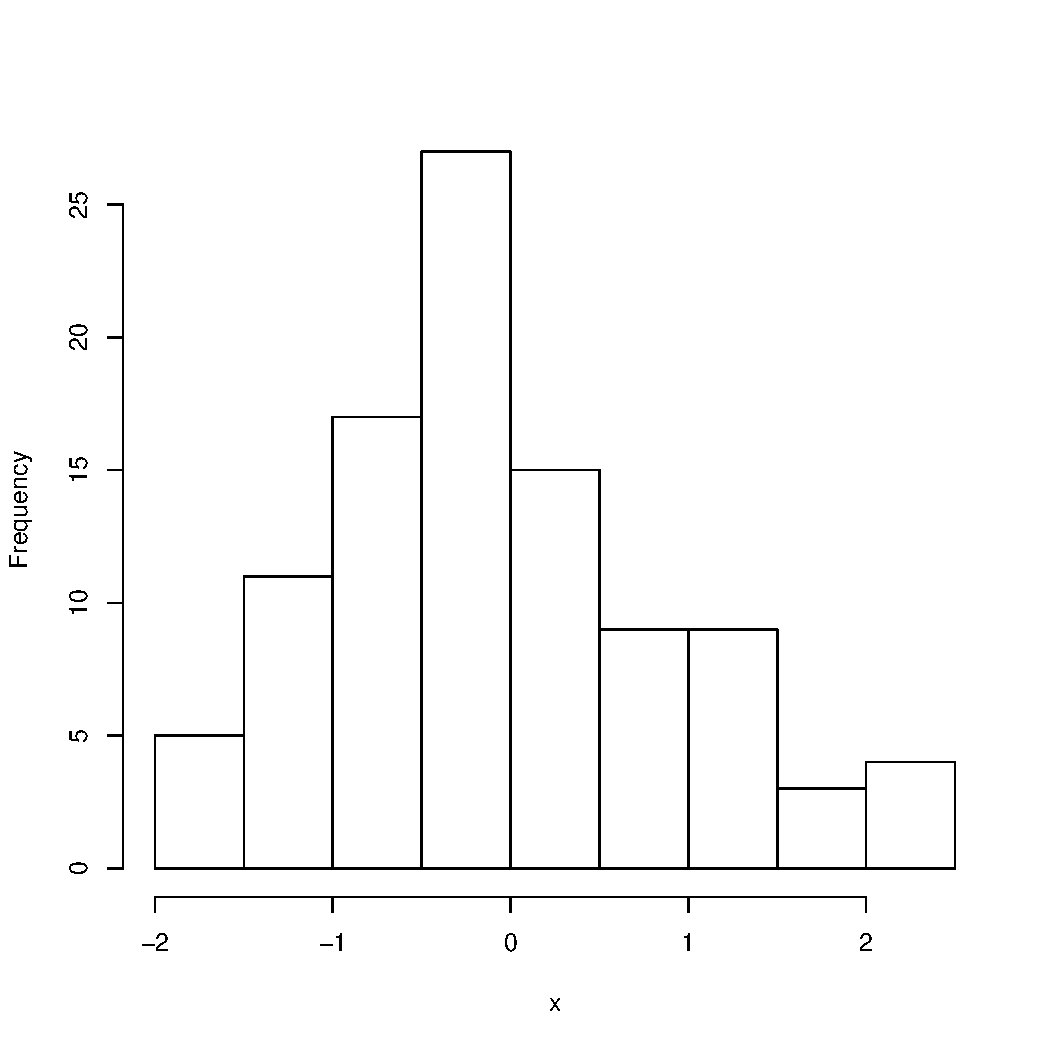
\includegraphics[width = 0.6\linewidth]{../fig/f_baseplot.pdf}
\end{frame}
\begin{frame}[fragile]
\frametitle{\texttt{ggplot2} plot (Org source)}
\label{sec-3-1-8}



\begin{verbatim}
 1:  #+headers: :exports results 
 2:  #+headers: :results graphics
 3:  #+headers: :file f_ggplot2_ex.pdf
 4:  #+begin_src R 
 5:  library(ggplot2)
 6:  x <- data.frame(var = rnorm(100))
 7:  ggplot(aes(x = var), data = x) 
 8:        + geom_histogram()
 9:  #+end_src 
10:  
11:  #+RESULTS:
12:  [[file:f_ggplot2_ex.pdf]]
\end{verbatim}
\end{frame}
\begin{frame}
\frametitle{\texttt{ggplot2} plot (evaluated)}
\label{sec-3-1-9}


 

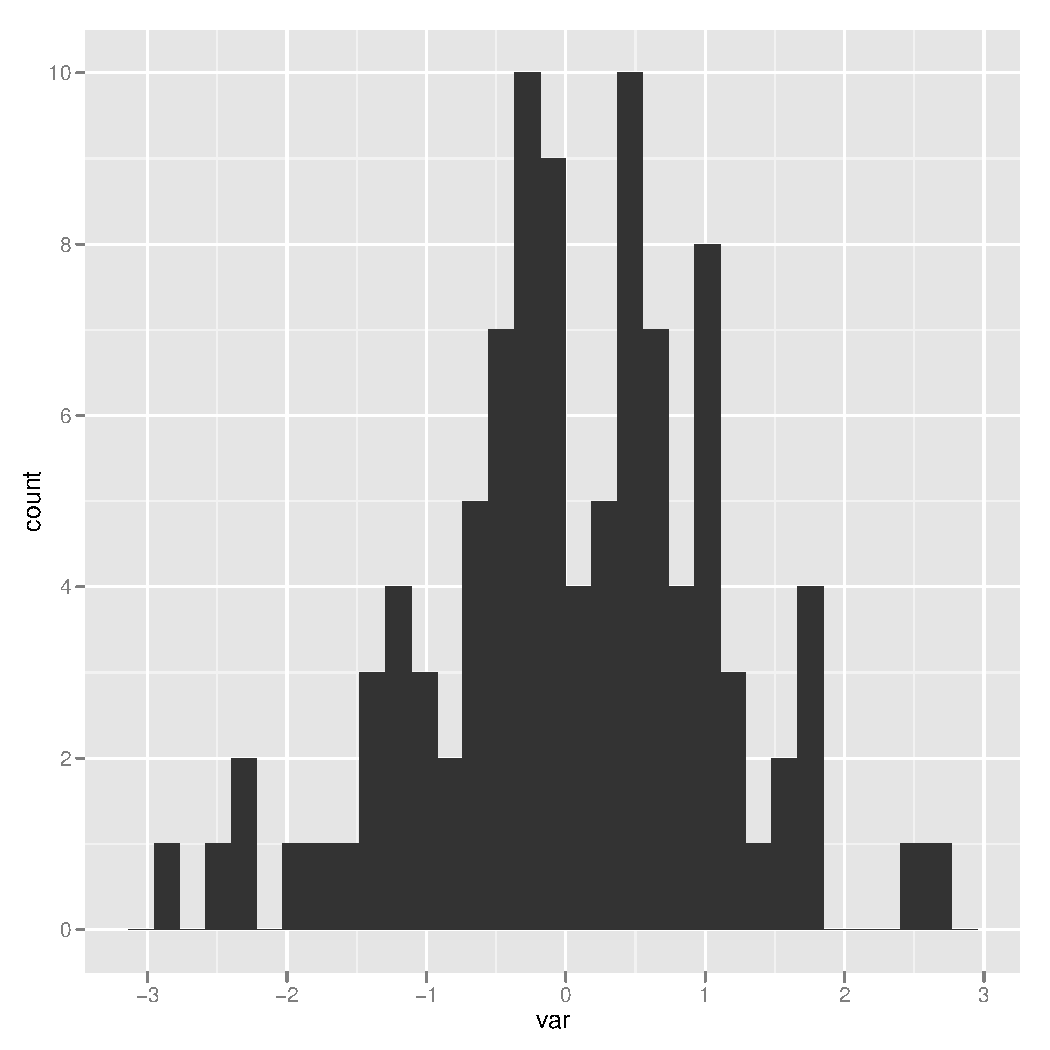
\includegraphics[width = 0.7\linewidth]{../fig/f_ggplot2_example.pdf}
\end{frame}
\subsection{Tangling und weaving}
\label{sec-3-2}
\begin{frame}
\frametitle{Tangling and weaving code}
\label{sec-3-2-1}


\begin{itemize}
\item \emph{Weaving} refers to the exportation of a mixed code/prose document to a format
  that can be read by a human (HTML, \LaTeX, Ascii, \ldots{}).
\item \emph{Tangling} means to extract only the code to a separate file
\end{itemize}

(Source: Schulte et al. 2012: 12)
\end{frame}
\begin{frame}[fragile]
\frametitle{Beispiel für \enquote{code tangling}}
\label{sec-3-2-2}



\begin{verbatim}
#+BEGIN_SRC R :tangle ../src/example_tangled.R 
## Comment: Assign value 1 to variable x
x <- 1
#+END_SRC
\end{verbatim}
\end{frame}
\begin{frame}[fragile]
\frametitle{Beispiel (Fortsetzung): Tangled R code}
\label{sec-3-2-3}


Hier ist der Inhalt der Datei \texttt{../src/example\_tangled.R}
\begin{block}{\texttt{../src/example\_tangled.R}}
\label{sec-3-2-3-1}

\begin{footnotesize}

\begin{verbatim}

## [[file:e:/projects/confer/ps2012-07-KRUG_org_r/slide/ps2012-07-KRUG_org_R.org::*Example%20of%20code%20tangling][Example-of-code-tangling:2]]

## Comment: Assign value 1 to variable x
x <- 1

## Example-of-code-tangling:2 ends here
\end{verbatim}
\end{footnotesize}
\end{block}
\end{frame}
\subsection{Ein kurzes vollständiges Org-Beispiel}
\label{sec-3-3}
\begin{frame}
\frametitle{Ein kurzes vollständiges Org-Beispiel}
\label{sec-3-3-1}


Siehe hierfür \texttt{pub/d\_example.org} and \texttt{pub/d\_example.pdf}.
\end{frame}
\section{R und andere Sprachen (Python)}
\label{sec-4}
\subsection{}
\begin{frame}[fragile,shrink = 10]
\frametitle{Chaining (source)}
\label{sec-4-1-1}




\lstset{language=org}
\begin{lstlisting}
Define variable =y= in a Python code block: 
#+name: chainexamp
#+begin_src python :results value :session *python*
y = 9**4
y
#+end_src

#+RESULTS: chainexamp
: 10000

Then pass variable =y= to an R code block:
#+BEGIN_SRC R :var x=chainexamp :session *R2*
print(x)
print(x*2)
#+END_SRC

#+RESULTS:
: [1] 6561
: [1] 13122
\end{lstlisting}
\end{frame}
\begin{frame}[fragile]
\frametitle{Chaining (evaluated)}
\label{sec-4-1-2}


Define variable \texttt{y} in a Python code block: 

\lstset{language=Python}
\begin{lstlisting}
y = 10**4
y
\end{lstlisting}

\begin{verbatim}
 10000
\end{verbatim}


Then pass variable \texttt{y} to an R code block:

\lstset{language=R}
\begin{lstlisting}
print(x)
print(x*2)
\end{lstlisting}

\begin{verbatim}
 [1] 10000
 [1] 20000
\end{verbatim}
\end{frame}
\section{Literatur/Quellen}
\label{sec-5}
\subsection{}
\begin{frame}
\frametitle{Literatur/Quellen}
\label{sec-5-1-1}


\begin{itemize}
\item Schulte, Eric, Dan Davison, Thomas Dye, und Carsten Dominik. 2012. A
  Multi-Language Computing Environment for Literate Programming and Reproducible
  Research. Journal of Statistical Software 46: 1–24.
\item \href{http://orgmode.org/worg/org-contrib/babel/how-to-use-Org-Babel-for-R.html}{http://orgmode.org/worg/org-contrib/babel/how-to-use-Org-Babel-for-R.html}
\end{itemize}
\end{frame}

\end{document}
